\documentclass{article}
\usepackage{122}

\usepackage{graphicx}

\title{Биоинформатика \\ Домашнее задание №4}

\graphicspath{ {./bio/shapes/} }

\begin{document}
  \maketitle

  \section{Выбранный ген}
  В прошлом задание у нас был ген \texttt{RNA polymerase RPB3}.
  Я нашёл его структуру для двух видов: \texttt{5IY6} для человека и \texttt{1I3Q} для дрожжей.

  \section{Задание №1}
  \subsection{Структура белка}
  Тут почему-то в структуре белка отображается ДНК, которую он будет копировать.
  Спрятать её у меня не получилось, но вроде и не надо.
  \begin{center}
    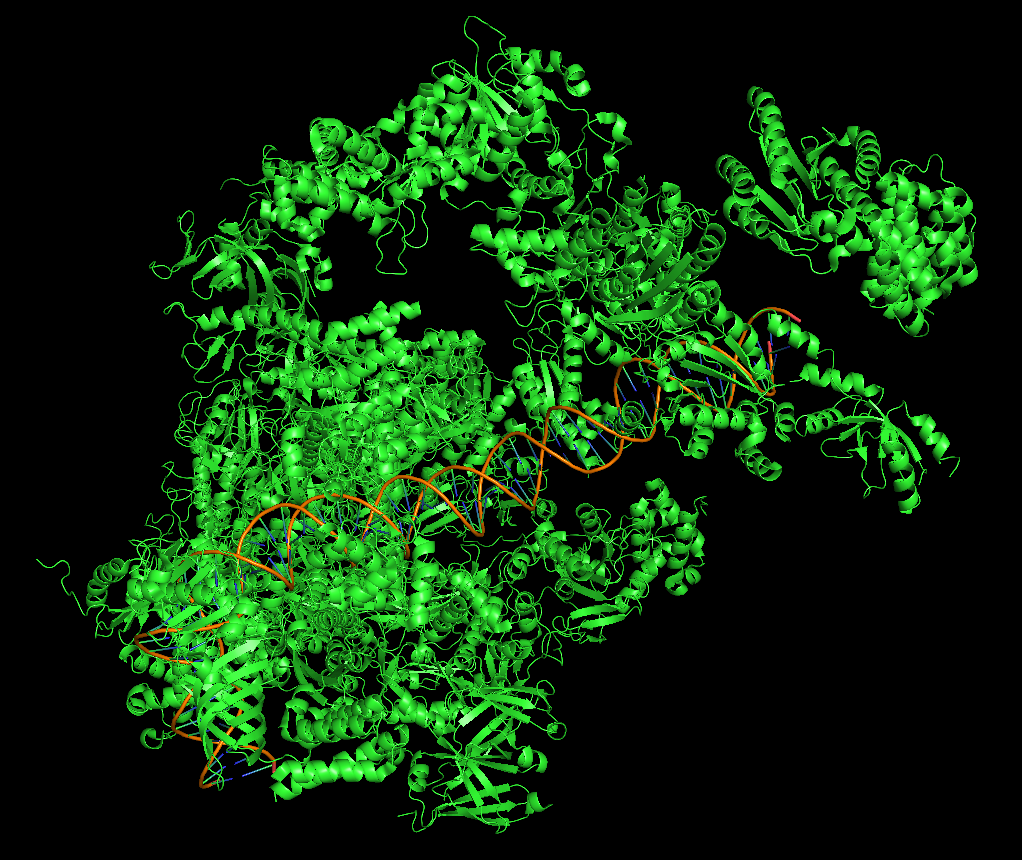
\includegraphics[width=.9\textwidth]{main.png}
  \end{center}

  \subsection{Выбранная спираль}
  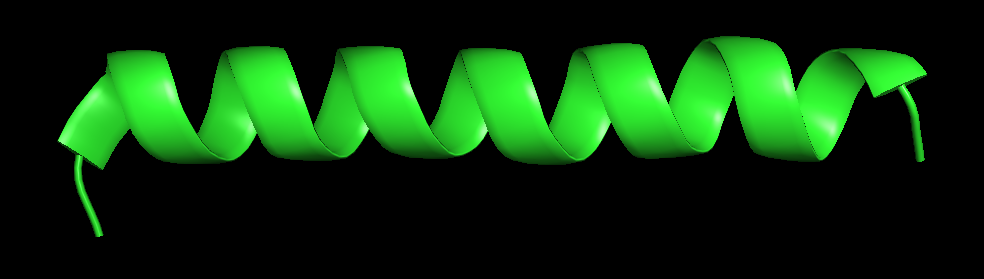
\includegraphics[width=\textwidth]{spiral.png}

  \subsection{С водородными связями}
  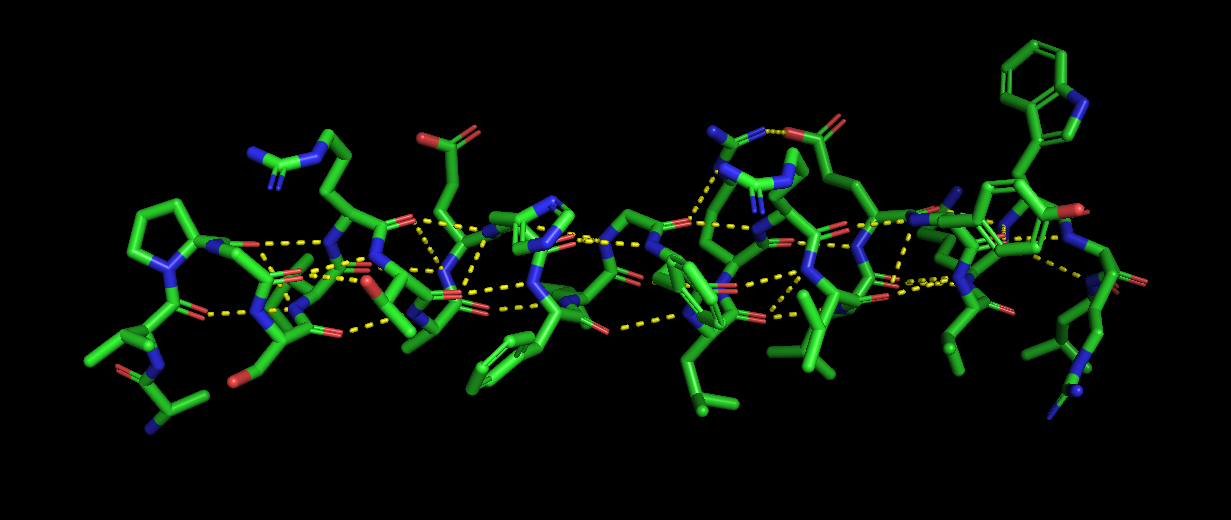
\includegraphics[width=\textwidth]{hbonds.png}

  \subsection{И их длинны}
  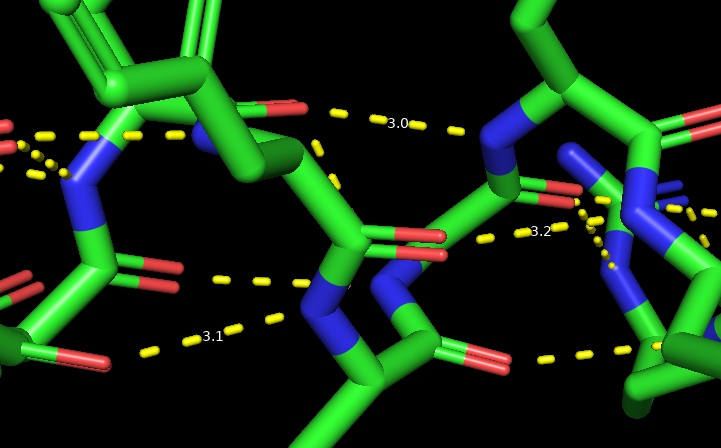
\includegraphics[width=\textwidth]{hbondlen.png}

  \subsection{Ответы на вопросы}
  \begin{enumerate}
    \item Между какими атомами (элемент) найдены связи? \\
      \textbf{Ответ:} кислород и азот
    \item Есть ли находки, которые вам кажутся странными? \\
      \textbf{Ответ:} нет
    \item Каковы их длины? \\
      \textbf{Ответ:} $3.0$, $3.1$ и $3.2$
    \item Отличаются ли от табличных? \\
      \textbf{Ответ:} нет
  \end{enumerate}

  \section{Задание №2}
  \subsection{Два белка}
  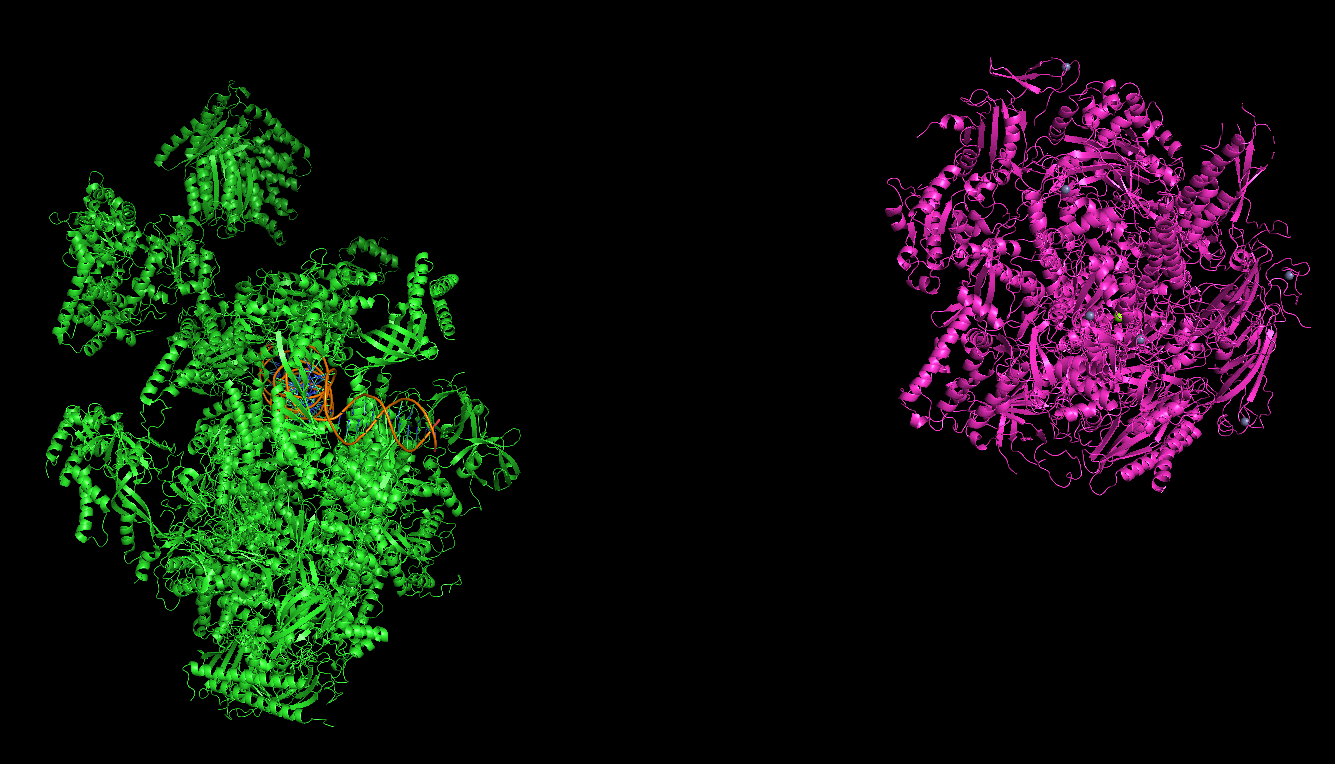
\includegraphics[width=\textwidth]{2.png}

  \subsection{Их выравнивание}
  \begin{center}
    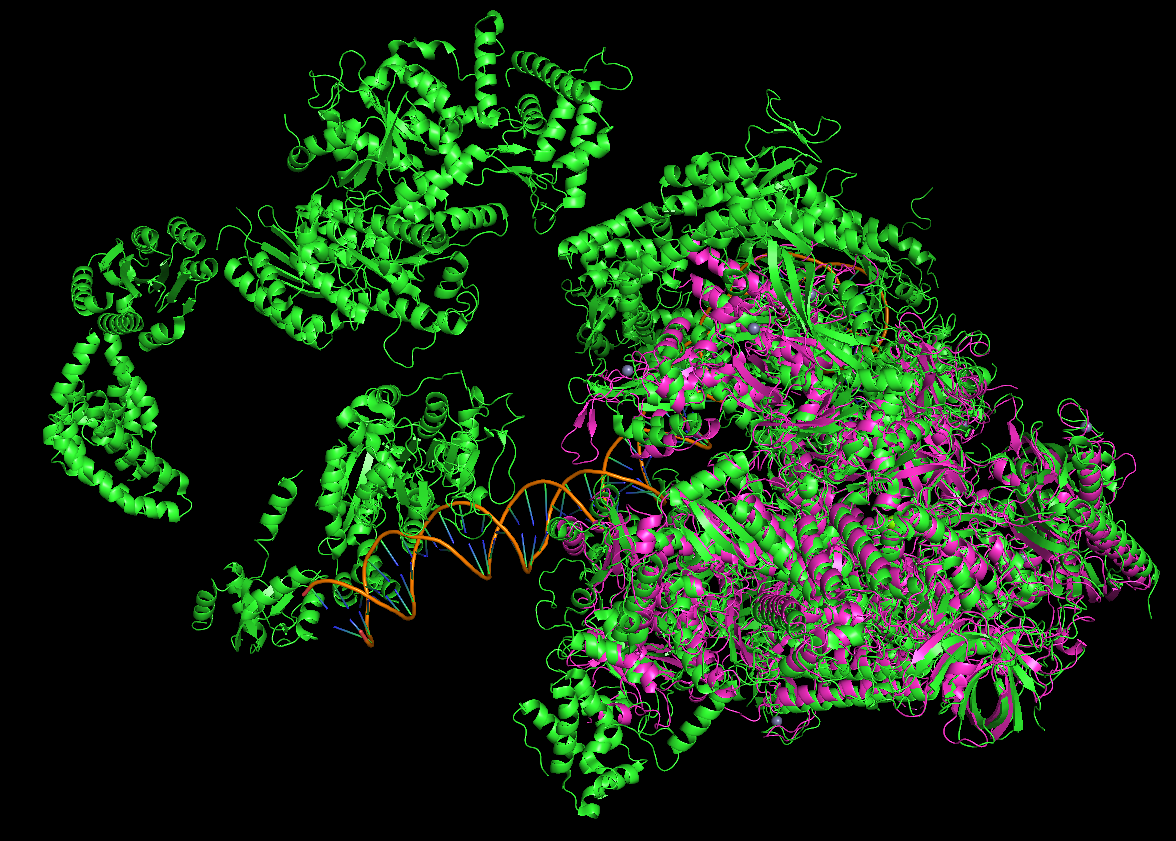
\includegraphics[width=.8\textwidth]{align.png} \\
    RMSD = $2.137$ ($19651$ atoms)
  \end{center}

  \subsection{Подсветка различий}
  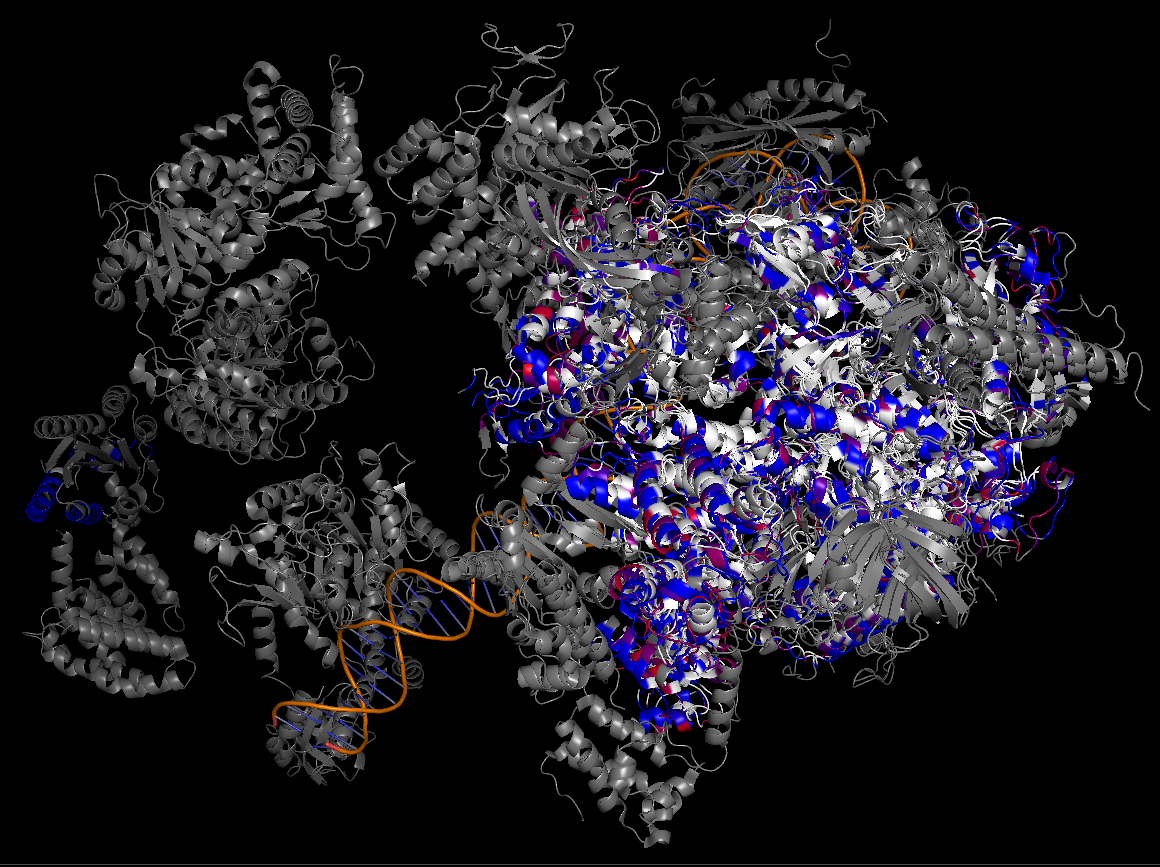
\includegraphics[width=\textwidth]{colorbig.png}
  \subsubsection{Вот маленький кусок отдельно}
  \begin{center}
    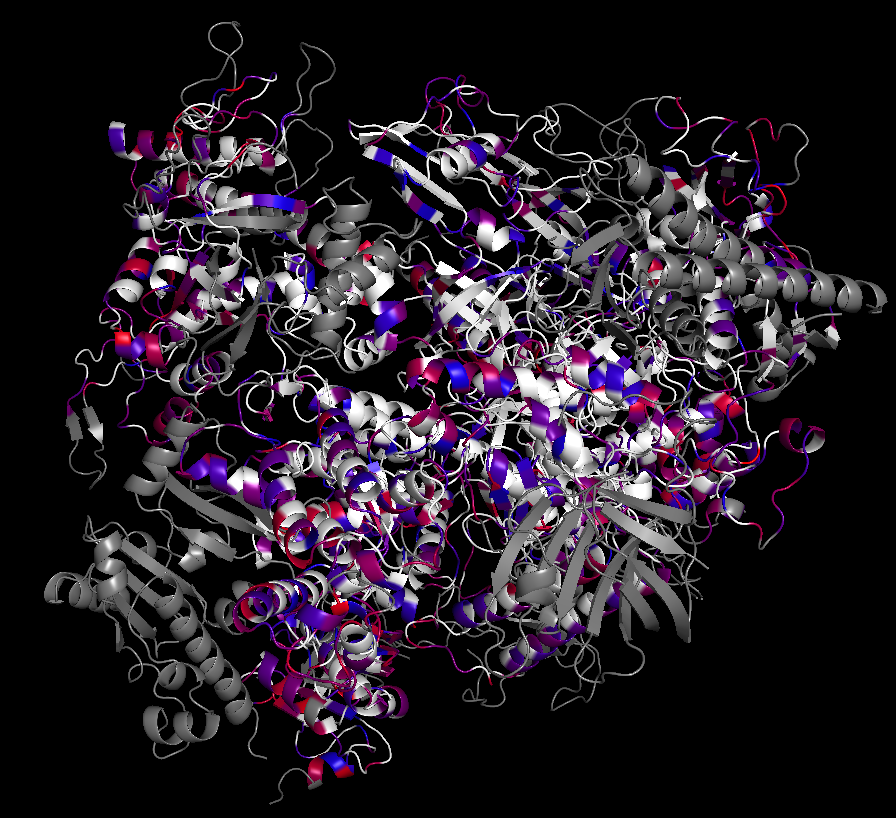
\includegraphics[width=.5\textwidth]{colorsmall.png}
  \end{center}

\end{document}
